% 通信系统述论
% LaTeX Template
% Version 1.0 
\documentclass[11pt]{ctexart} % 默认为5号(pt=10.5)字体,pt12为小四
\linespread{1.3} % 行距为1.3
\usepackage{url}  % 使用宏包url提供超链接
\usepackage{graphicx}
\usepackage[top=1.8cm, bottom=2.5cm, left=2.5cm, right=2.5cm]{geometry}  % 使用geometry来控制页面布局
\title{\centering {\LARGE{通信系统述论}}\\% Title
} % Subtitle
\author{\textsc \small{{陈李锋 14通信 2014081025 }} % Author
} % Institution

%----------------------------------------------------------------------------------------

\begin{document}

\maketitle % Print the title section

\begin{abstract} %摘要
通信系统,随着现代的发展,普遍认为指的就是计算机网络系统。因为许多传统古老的通信系统(如寄信,无线电报)在越发不重要或逐渐消失,而三网融合(电信网、广播电视网、互联网)又是网络发展的趋势,所以现在通信系统的发展实际上就是计算机网络的发展。在这个发展过程中,计算机网络系统结构(Computer Network Architecture)显得越来越重要,其指的是个分层次的模块式结构。网络结构的发展是从传统的第一个标准化的计算机网络互连体系结构OSI/RM(Open System Interconnection ReferenceModel,开放系统互连参考模型),发展到TCP/IP协议体系结构(又称TCP/IP协议参考模型)的过程。本文遵从这个顺序,简单介绍通信系统,也就是计算机网络系统的发展。
\\\\关键词: 计算机网络\quad  通信系统\quad OSI/RM \quad TCP/IP 

\end{abstract}

\subsubsection*{\raggedleft{计算机网络系统分层次结构}}
\paragraph{}
分层次的模块式结构,这样设计的目的一方面是便于我们从宏观上把握整个网络体系架构,实现快速分析与排除网络故障;另一方面是便于程序开发人员在进行网络系统开发时针对不同网络功能进行独立开发,无须考虑其他层的功能。

另外,在分层结构中,无论哪一种计算机网络体系结构,也无论是体系结构中的哪一层,都不是针对具体的设备或者具体的软件而言的,而只是针对每层中所要实现的网络服务功能来划分的。因为每一层所代表的是一组网络功能,而实现某一个功能又可以有许多不同的软/硬件方案。如物理层上就可以有许多不同的传输介质(如同轴电缆、双绞线、光纤等)和网络设备(如集线器、中继器),当然还有许多对应的通信协议。其他各层也一样。计算机网络中的软/硬件是计算机网络通信和数据传输的实体,也就是网络任务的具体执行者。

有了这样一个结构模型,就把整个计算机网络软、硬件技术和设备串起来了,所有软、硬件技术都围绕在这个中心周围。
\begin{itemize}
\item 同一层中的各网络节点都有相同的层次结构,具有同样的功能。
\item 同一节点内相邻层之间通过接口(可以是逻辑接口)进行通信。
\item 每一层使用下一层提供的服务,并向其上层提供服务
\end{itemize}



\subsubsection*{\raggedleft{OSI/RM体系结构}}
\paragraph{}
 OSI/RM体系结构是第一个标准化的计算机网络体系结构。它是针对广域网通信(也就是不同网络之间的通信)进行设计的,将整个网络通信的功能划分为七个层次,由低到高分别是物理层(PhysicalLayer)、数据链路层(DataLinkLayer)、网络层(NetworkLayer)、传输层(Transport Layer)、会话层(Session Layer)、表示层(PresentationLayer)、应用层(Application Layer)。
 
 但任何广域网其实都是由多个远程局域网连接而成的,所以在OSI/RM中不仅包括了广域网中不同局域网间通信的功能层次(上面五层),也给出了局域网内通信所必需的两个层次(最下面两层)。OSI/RM低四层(从物理层到传输层)定义了如何进行端到端的数据传输,也就是定义了如何通过网卡、物理电缆、交换路由器进行数据传输;而高三层(从会话层到应用层)定义了终端系统的应用程序和用户如何彼此通信,也即定义了如何重建从发送方到目的方的应用程序数据流。更多的是把OSI/RM的七层结构分成低三层和高四层的,低三层负责创建网络通信所需的网络连接(面向网络),属于“通信子网”部分,高四层具体负责端到端的用户数据通信(面向用户),属于“资源子网”部分。OSI/RM结构中各层功能如下图所示。
 
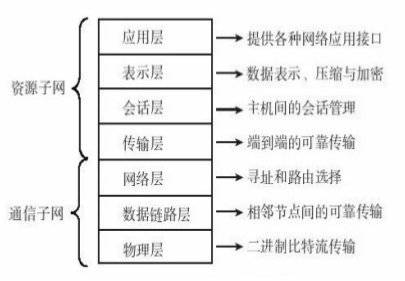
\includegraphics[width=0.7\linewidth]{OSI-RM}

但是OSI/RM的七层结构划分从现在看来,并不是很科学,这主要表现在两方面:一是层次数方面还是多了些;二是在进行网络系统设计时仍然觉得比较麻烦。另外,像“会话层”和“表示层”单独划分的意义并不大,因为它们的用途并不像其他层那样明显。所以在后面的TCP/IP协议体系结构中,不再有这两层了。

\subsubsection*{\raggedleft{TCP/IP体系结构}}
\paragraph{}
TCP/IP协议体系结构(又称TCP/IP协议参考
模型)是专门针对使用TCP/IP协议簇的广域计算
机网络而开发的,可以说是OSI/RM的改进版本。
但绝不能简单地认为是改进版,因为它与OSI/RM
所针对的网络类型存在较大区别,所以这两种体
系结构中各层所采用的通信协议,以及功能实现
原理上都存在非常大的差异。现在我们常用的通信协
议,绝大多数都不是很适用于OSI/RM,而是适用
于TCP/IP协议体系结构,因为它们都是应用于
TCP/IP网络中。

TCP/IP协议体系结构起源于20世纪60年代
末,首先由美国国防部高级研究规划署(DARPA)作为
其研究的一部分,所以又称DARPA参考模型。现在使用最广的Internet也是基于这一模型
设计的,因为目前的Internet基本上都是采用
TCP/IP协议簇的,包括我们企业内部局域网。
TCP/IP协议体系结构只划分了四层,从高到
低分别是:应用层(Apllication Layer)、传输层
(TransportLayer)、网际互连层(InternetLayer,又称互联网层)和网络访问层(Network
Access Layer,又称网络接入层、网络接口层)。虽然只有四层,但它却包含了
OSI/RM中的所有七层的功能,同样包括了局域网
和广域网通信所需要的全部功能。下图描绘了
TCP/IP协议体系结构与OSI/RM层次间的关系。

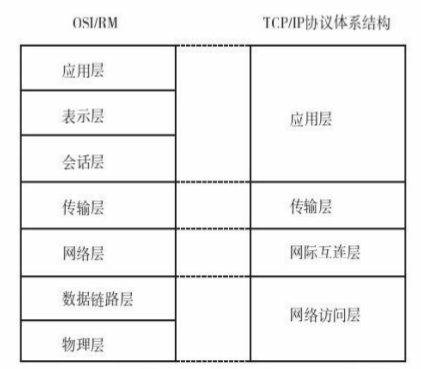
\includegraphics[width=0.7\linewidth]{OSI&TCP}

从图中可以看出,在TCP/IP协议体系结构中
对原来OSI/RM的七层结构进行了进一步的简化,
主要体现在以下两个方面:

*把原来的“物理层”和“数据链路层”这两层
结构合并为一层,即网络访问层,它提供局域网
中的功能;

*合并了原来OSI/RM中的最高的三层,成为
新的应用层。因为事实上,在OSI/RM中会话层和
表示层的功能都非常单一,完全可以合并到应用
层之中。


总体而言,TCP/IP协议体系结构更加精简,
更有利于网络系统的设计。但是其中网络访问层
本身并不是实际的一层,包括了OSI/RM中的物理层和数据链路层这两层的功能,现在把它们其实
合并不是很合理,所以现在通常认为TCP/IP五层(网络访问层也分为OSI/RM 的数据链路层物理层)网络体系结构才是最
为科学、合理的。因为它综合了OSI/RM和TCP/IP
协议两种体系结构的优点,同时克服了这两种体
系结构的不足。
\subsubsection*{OSI/RM和TCP/IP协议体系结构的比较}
  TCP/IP协议体系结构是在OSI/RM基础上,专
门针对TCP/IP网络而开发的体系结构,所以它既
有OSI/RM的基本模型结构和层次划分思想,又针
对了特定的TCP/IP网络,所以其更加具体化,更
加具有可操作性。

相同之处
\begin{itemize}
\item 层次结构划分思想相同:都是以协议栈(不同协议形成的层次结构)为基础进行层次结构划分的
% 这两种体系结构都是以协议栈(不同协议形成的层次结构)为基础进行层次结构划分的,并且协议栈中的协议是彼此独立的。
\item 总体层次结构相似
% 在这两个体系结构中,虽然总的层数和对应层次名称都有所不同,但总体层次结构还是极其相似的。
\end{itemize}

不同之处
\begin{itemize}
\item 适用范围不同:OSI/RM是一个理想化的模型,TCP/IP协议体系结构仅适用于TCP/IP类型网络
\item 层次结构不同:具体上面已经说
\item 支持的网络通信模式不同:OSI/RM的网络层同时支持无连接和面向连接的网络通信,TCP/IP模型的网络层只提供无连接的服务
\item 所包括的通信协议不同:TCP/IP网络中的通信协议是专门针对具体的TCP/IP协议体系结构而开发的,而OSI/RM是一种开放型的
\end{itemize}


参考文献:

[1]OSI七层与TCP/IP五层网络架构详解.www.ha97.com  \url{ http://www.ha97.com/3215.html} 

[2] TCP/IP/. wikipedia. \url{https://en.wikipedia.org/wiki/Transmission_Control_Protocol}

[3] 传输控制协议.wikipedia.  \url{https://zh.wikipedia.org/wiki/传输控制协议}

[4] 王达.深入理解计算机网络. 机械出版社. 北京.2013


\end{document}
